\documentclass[12pt]{article}
\usepackage[margin=1in]{geometry}
\usepackage[pdftex]{graphicx}
\usepackage{multirow}
\usepackage{setspace}
\usepackage{enumitem}
\pagestyle{plain}

\begin{document}

\noindent
% Course information
\begin{tabular*}{\textwidth}{l @{\extracolsep{\fill}} r}
  & \multirow{3}{*}{
\includegraphics[height=1.0in]{logo.jpg}} \\
  \large Comp. Phys. Lab for Statistical Mechanics & \\
  \large Fall Quarter 2025 & \\
  \large Physics 112L & \\
\end{tabular*}
\vspace{10mm}

\noindent
% Professor information
\begin{tabular}{ l l }
  \multirow{6}{*}{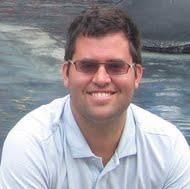
\includegraphics[height=1.25in]{mike.jpg}} & \\
  & \\
  & Michael Mulhearn \\
  & mulhearn@physics.ucdavis.edu \\
  & Physics 317 \\
  & \\
\end{tabular}
\vskip 0.5cm

\noindent
\begin{tabbing}
\hspace*{8em} \= \kill 
\textbf {Lecture:} \> Tuesday 2:10-3:00 PM in Roessler 55 \\
\end{tabbing}
\noindent
\begin{tabbing}
\hspace*{8em} \= \kill 
\textbf{Textbooks:} \> Thermal Physics by Daniel V. Schroeder (any volume)\\
\> ~~~(Recommended for reference, or any other Intro. Stat Mech text.)\\
\> Lecture notes on Scientific Python (link on course site)\\
\end{tabbing}
\noindent
\begin{tabbing}
\hspace*{8em}\= \hspace*{10em} \= \kill 
\textbf{Course TA:}
\> Cameron Chaffey \> crchaffey@ucdavis.edu \\
\end{tabbing}
\noindent
\begin{tabbing}
\hspace*{8em}\= \hspace*{10em} \= \kill 
\textbf{Office Hours:}
    \> Mulhearn: \> TBD \\
    \> Chaffey:  \> TBD \\
\end{tabbing}
\noindent
\begin{tabbing}
\hspace*{12em}\= \kill 
\textbf{Exams/Quizzes:} \> None planned, but see caveats in the plagiarmism section.\\
\textbf{Final Project:} \> Due December, 10 2025 10:30 AM\\
\end{tabbing}


\noindent
\textbf {Course Description:}\\
Applications of computational physics to problems from Statistical
Mechanics.  Application of numerical techniques, and comparison to
analytic solutions (where they exist).\\[8pt]

\noindent
\textbf {System of Units:}\\
To receive any credit, your solutions must adopt the system of units
as presented in lecture and in the write-up for each assignment.  The
system of units must be used throughout your solution.  You may not
e.g. do the calcuation in SI and then convert to our system of units
later.\\[8pt]

\noindent
\textbf {Plagiarism and Academic Conduct:}\\
You must adhere to the UC Davis Code of Academic Conduct, available
online at ossja website. In particular, you may not take credit for
any work not created by you.  {\bf You may not direct search engines,
  generative AI tools, homework help websites, or other external
  resources toward the specific problems that are assigned to you.}
If you do, then you must disclose it, and you will receive a zero for
the entire assignment.  If you do not disclose it, and are caught,
then you will fail the entire course.\\[3pt]

\noindent
You are allowed to collaborate with other students in the course,
including discussing specific problems in the homework, unless you
have reason to believe the students are using unauthorized methods.
The solution that you provide must be your own: each and every line.
In general, you should be able to explain why each line in your code
is there.  If you do not understand something in your solution because
you relied on trial and error, then you should state that in the
comments, including explaining any other things that you tried.  For
example:
\begin{verbatim}
# I don't understand why this factor of two is needed
# I have included it because it gives the correct result:
\end{verbatim}

\noindent
If I become suspicous that plagarism or cheating is occurring, I
reserve the right to add quizes, exams, or other means of grading.
You should always be prepared to explain your code if asked.\\[3pt]

\noindent
\textbf {Course Philosophy:}\\
Computational physics is essential to nearly every career related to
physics.  Unfortunately, the educational pipeline, since grade school,
does not adequately prepare students with programming skills, and so a
central feature of computational physics courses is a wide
distribution of student programming abilities.  There are students
that are better programmers than most physics professors, students
that have little practice outside of the required computational
courses, and everything in between.\\[3pt]

\noindent
Fortunately, in this course we are concerned with {\bf computational
  physics} and not just {\bf computer programming}.  You do not need
to be an expert computer programmer to succeed in this course. You do
need to gain enough programming competency to handle the fascinating
physics problems we will tackle.  {\bf The primary objective of this
  course is to make you confident in using programming independently
  as an essential and effective tool for solving physics
  problems.}\\[3pt]

\noindent
This is a one unit course, and I will do my best to keep the workload
appropriate.  However, given the wide variation in student programming
abilities, inevitably some students will find the homework more
time-consuming than others.  If you do find yourself working longer on
the assignments, please understand that this is time well-spent:
gaining more proficiency in computing is almost certainly one of the
best possible uses of your time at this stage in your career.  There
are a vanishing small number of physics-related career options that do
not require programming ability.\\[3pt]

\noindent
\textbf{Homework:}\\
There will be up four home-work assignments which will feature problems in computational physics.\\[3pt]

\noindent
\textbf{Final Project:}\\ In lieu of a final exam, you will design an
independent creative problem.  While your particular problem may have
already been solved online, your solution should vary substantially
from anything available online.\\[3pt]

\noindent
\textbf {Grades:}\\
Final grades will be approximately $80\%$ Homework and $20\%$ Final Project.  You will be allowed to submit one homework assignment late, but you must complete every assignment and your final project to complete the course.\\

\end{document}

